\documentclass{article}\usepackage[]{graphicx}\usepackage[]{color}
%% maxwidth is the original width if it is less than linewidth
%% otherwise use linewidth (to make sure the graphics do not exceed the margin)
\makeatletter
\def\maxwidth{ %
  \ifdim\Gin@nat@width>\linewidth
    \linewidth
  \else
    \Gin@nat@width
  \fi
}
\makeatother

\definecolor{fgcolor}{rgb}{0.345, 0.345, 0.345}
\newcommand{\hlnum}[1]{\textcolor[rgb]{0.686,0.059,0.569}{#1}}%
\newcommand{\hlstr}[1]{\textcolor[rgb]{0.192,0.494,0.8}{#1}}%
\newcommand{\hlcom}[1]{\textcolor[rgb]{0.678,0.584,0.686}{\textit{#1}}}%
\newcommand{\hlopt}[1]{\textcolor[rgb]{0,0,0}{#1}}%
\newcommand{\hlstd}[1]{\textcolor[rgb]{0.345,0.345,0.345}{#1}}%
\newcommand{\hlkwa}[1]{\textcolor[rgb]{0.161,0.373,0.58}{\textbf{#1}}}%
\newcommand{\hlkwb}[1]{\textcolor[rgb]{0.69,0.353,0.396}{#1}}%
\newcommand{\hlkwc}[1]{\textcolor[rgb]{0.333,0.667,0.333}{#1}}%
\newcommand{\hlkwd}[1]{\textcolor[rgb]{0.737,0.353,0.396}{\textbf{#1}}}%
\let\hlipl\hlkwb

\usepackage{framed}
\makeatletter
\newenvironment{kframe}{%
 \def\at@end@of@kframe{}%
 \ifinner\ifhmode%
  \def\at@end@of@kframe{\end{minipage}}%
  \begin{minipage}{\columnwidth}%
 \fi\fi%
 \def\FrameCommand##1{\hskip\@totalleftmargin \hskip-\fboxsep
 \colorbox{shadecolor}{##1}\hskip-\fboxsep
     % There is no \\@totalrightmargin, so:
     \hskip-\linewidth \hskip-\@totalleftmargin \hskip\columnwidth}%
 \MakeFramed {\advance\hsize-\width
   \@totalleftmargin\z@ \linewidth\hsize
   \@setminipage}}%
 {\par\unskip\endMakeFramed%
 \at@end@of@kframe}
\makeatother

\definecolor{shadecolor}{rgb}{.97, .97, .97}
\definecolor{messagecolor}{rgb}{0, 0, 0}
\definecolor{warningcolor}{rgb}{1, 0, 1}
\definecolor{errorcolor}{rgb}{1, 0, 0}
\newenvironment{knitrout}{}{} % an empty environment to be redefined in TeX

\usepackage{alltt}
\usepackage{Sweave}
\usepackage{float}
\usepackage{graphicx}
\usepackage{tabularx}
\usepackage{siunitx}
\usepackage{amssymb} % for math symbols
\usepackage{amsmath} % for aligning equations
\usepackage{textcomp}
\usepackage{mdframed}
\usepackage{natbib}
\bibliographystyle{..//bib/styles/besjournals.bst}
\usepackage[small]{caption}
\setlength{\captionmargin}{30pt}
\setlength{\abovecaptionskip}{0pt}
\setlength{\belowcaptionskip}{10pt}
\topmargin -1.5cm        
\oddsidemargin -0.04cm   
\evensidemargin -0.04cm
\textwidth 16.59cm
\textheight 21.94cm 
%\pagestyle{empty} %comment if want page numbers
\parskip 7.2pt
\renewcommand{\baselinestretch}{1.5}
\parindent 0pt
\usepackage{lineno}
\linenumbers

\newmdenv[
  topline=true,
  bottomline=true,
  skipabove=\topsep,
  skipbelow=\topsep
]{siderules}

%% R Script


\IfFileExists{upquote.sty}{\usepackage{upquote}}{}
\begin{document}
\noindent \textbf{\Large{Regional Risk Outline}}

\noindent Authors:\\
C. J. Chamberlain $^{1,2}$, B. I. Cook $^{3}$, I. Morales Castilla $^{1,4}$ \& E. M. Wolkovich $^{1,2}$
\vspace{2ex}\\
\emph{Author affiliations:}\\
$^{1}$Arnold Arboretum of Harvard University, 1300 Centre Street, Boston, Massachusetts, USA; \\
$^{2}$Organismic \& Evolutionary Biology, Harvard University, 26 Oxford Street, Cambridge, Massachusetts, USA; \\
$^{3}$NASA Goddard Institute for Space Studies, New York, New York, USA; \\
$^{4}$Edificio Ciencias, Campus Universitario 28805 Alcalá de Henares, Madrid, Spain \\
\vspace{2ex}
$^*$Corresponding author: 248.953.0189; cchamberlain@g.harvard.edu\\

\renewcommand{\thetable}{\arabic{table}}
\renewcommand{\thefigure}{\arabic{figure}}
\renewcommand{\labelitemi}{$-$}
\setkeys{Gin}{width=0.8\textwidth}

%%%%%%%%%%%%%%%%%%%%%%%%%%%%%%%%%%%%%%%%%%%%%%%
%%%%%%%%%%%%%%%%%%%%%%%%%%%%%%%%%%%%%%%%%%%%%%%

%%%%% 1) PIECE TOGETHER THE PUZZLE! %%%%%
%%%%% 2) FORMULATE QUESTIONS %%%%%
%%%%% 3) ONCE THE INTRO IS SOLID, THEN MOVE ON TO METHODS! %%%%%%


\section*{Introduction}
\begin{enumerate}
\item Temperate tree and shrub species are at risk of damage from late spring freezing events, also known as false springs.
\begin{enumerate}
\item The growing season is lengthening across many regions in the northern hemisphere \citep{Chen2005, Liu2006, Kukal2018}, but last spring frosts still pose a threat in many of these regions \citep{Wypych2016a}.
\item Due to the changing climate, spring onset is advancing and many temperate tree and shrub species are initiating leafout 4-6 days earlier per $^{\circ}$C of warming \citep{Wolkovich2012, IPCC2014}.
%\item With climate change advancing, this interaction of cues may shift spring phenologies both across and within species. 
\item However, last spring freeze dates are not predicted to advance at the same rate as spring onset in some regions of the world \citep{Inouye2008, Martin2010, Labe2016, Sgubin2018}, potentially amplifying the effects of false spring events in these regions.
\item In Germany, for example, the last freeze date has advanced by 2.6 days per decade since 1955 \citep{Zohner2016}.
\item Major false spring events have been recorded in recent years and have found it can take 16-38 days for trees to refoliate \citep{Gu2008, Augspurger2009, Augspurger2013, Menzel2015}, which can detrimentally affect crucial processes such as carbon updake and nutrient cycling \citep{Hufkens2012, Richardson2013, Klosterman2018}.
\end{enumerate}


\item Plant phenology, which is defined as the timing of recurring life-history events such as budburst, strongly tracks shifts in climate \citep{Cleland2007, Wolkovich2012}.
\begin{enumerate}
\item Episodic frosts are one of the largest limiting factors in species range limits \citep{Kollas2014}.
\item Temperate plants are exposed to freezing temperatures numerous times throughout the year, however, individuals are most at risk to damage from stochastic spring frosts, when frost tolerance is lowest \citep{Sakai1987}.
\item Individuals that initiate budburst and have not fully leafed out before the last spring freeze are at risk of leaf tissue loss, damage to the xylem, and slowed canopy development \citep{Gu2008, Hufkens2012}.
\item False spring events can result in photosynthetic tissue loss, which could potentially impact multiple years of growth and, with the growing season extending, individuals could be exposed to more frosts in the future \citep{Liu2018}.
\item Frost tolerance greatly diminishes once individuals exit the dormancy phase (i.e. processes leading to budburst) through full leaf expansion \citep{Vitasse2014, Lenz2016}.
\item Individuals that initiate budburst earlier in the season are more frost resistant \citep{Korner2016}, however, as climate change advances, less frost resistant individuals may start initiating budburst before the last freeze date.
\item Despite the importance of false spring events, the extent of damage and the frequency and intensity of false spring events is still largely unknown.
%\item Trees and shrubs in temperate regions optimize growth by using three cues to initiate budburst: low winter temperatures, warm spring temperatures, and increasing spring daylengths.
\end{enumerate}


%\item Temperate plants have evolved to minimize false spring damage through a myriad of strategies, with the most effective being avoidance: plants must exhibit flexible spring phenologies in order to maximize growth and minimize frost risk by timing budburst effectively \citep{Polgar2011, Basler2014}.
%\begin{enumerate}
%\item Plants growing in forest systems tend to exhibit staggered days of budburst.
%\item Lower canopy species typically initiate budburst earlier in the season in order to utilize available resources such as light, whereas larger canopy species usually initiate budburst later in the season.
%\item Thus, there is a trade-off between growing season length and frost risk. 

%\end{enumerate}

%\item Many studies have assessed the interplay between cue interactions and budburst dates by investigating potenital latitudinal effects \citep{Partanen2004, Viheraaarnio2006, Caffarra2011, Zohner2016, Gauzere2017}.
%\begin{enumerate}
%\end{enumerate}


\item There is large debate over whether or not spring freeze damage will increase \citep{Hannenin1991, Augspurger2013, Labe2016}, remain the same \citep{Scheifinger2003} or even decrease \citep{Kramer1994} with climate change.
\begin{enumerate}
\item Some research suggests false spring incidence has declined in many regions (i.e. across parts of North America and Asia), however the prevalence of spring frosts has consistently increased across Europe since 1982 \citep{Liu2018}.
\item However, recent studies have demonstrated regional effects may be more closely related to false spring risk: whether via altitudinal variation \citep{Vitra2017} or distance from the coast \citep{Wypych2016a}.
\item By better understanding these regional climatic implications, we may be able to determine which regions may be at risk currently and which regions may become more at risk in the future.
\end{enumerate}

\item The North Atlantic Ossilation (NAO) index is often used to describe winter and spring circulation across Europe.
\begin{enumerate}
\item More positive NAO phases tend to result in higher than average winter and early spring temperatures, and with climate change, higher NAO phases has correlated to even earlier budburst dates in some regions \citep{Chmielewski2001}, however it is unclear if more positive NAO phases also translates to more false springs.
\end{enumerate}

\item By improving and identifying budburst and climate trends in recent years, we could potentially amplify our predictability of future projections in false springs.
\begin{enumerate}
\item For this purpose, we assessed the number of false springs that occured across 11,684 sites around Europe, spanning altitudinal and coastal gradients, using observed phenological data (1,082,740 observations) for six temperate, deciduous trees and combined that with daily gridded climate data for each site that extended from 1951-2016. %% Do we want a table here with a breakdown of sites, species, and years? Probably in the supplement? 
\item In this study, a false spring was tallied when temperatures fell below -2.2$^{\circ}$ \citep{Schwartz1993} between budburst and leafout (CITE Rethinking here?)
\item We predicted that: (1) Earlier budburst species would experience more false springs, especially after 1983 and (2) there would be different regional effects on false spring incidence and those trends would shift when coupled with the effects of climate change.
\end{enumerate}
\end{enumerate}
%% WHERE DOES THIS GO? \item By using only gridded climate data from March 1st until June 30th, we compared the first half of our data (1951-1983) to the latter half (1984-2016) and found that some regions experienced increased exposure to false spring conditions, whereas many regions experienced fewer or similar conditions (Figure \ref{fig:region}). %% supplement?

\section*{Methods}
\subsection*{Phenological Data and Calculating Vegetative Risk}
\begin{enumerate}
\item We obtained phenological data from the Pan European Phenology network (PEP725, www.pep725.edu), which provides open access phenology records across Europe \citep{Templ2018}.
\item Since plants are most susceptible to damage from frost between budburst and full leafout, we selected only leafout data \citep[i.e., in][BBCH 11, which is defined as the point of leaf unfolding and the first visible leaf stalk]{Meier2001} from the PEP725 dataset.
\item We then subtracted 12 days from the leafout date to establish a rough estimate for day of budburst \citep{Donnelly2017}. 
\item The species used in the study were \textit{Aesculus hippocastanum L.}, \textit{Alnus glutinosa} (L.) Gaertn., \textit{Betula pendula} Roth., \textit{Fagus sylvatica} Ehrh., \textit{Fraxinus excelsior} L., \textit{Quercus robur} L.
\item Selection criteria for the species were as follows: (1) to be temperate, deciduous species that were not cultivars or used for crops, (2) there were at least 140,000 observations of BBCH 11, (3) to represent over half of the total number of sites available (11,684), (4) there were observations for at least 65 out of the 66 years of the study (1951-2016). % Do we want a table here with a breakdown of data for the supplement?
\end{enumerate}
\subsection*{Climate Data}
\begin{enumerate}
\item We collected daily gridded climate data from the European Climate Assessment \& Dataset (ECA\&D) and used the E-OBS 0.25 degree regular latitude-longitude grid from version 16. 
\item We used the daily minimum temperature dataset to determine if a false spring occurred.
\item False springs in this study were defined as temperatures at or below -2.2$^{\circ}$C \citep{Schwartz1993}.
\item In order to capture regional climatic effects we calculated the mean spring temperature by using the daily mean temperature from February 1 through April 30.
\item Mean spring temperature was calculated -- likely after chilling was accummulated -- in an attempt to incorporate a the general effects of spring forcing temperatures in our Bayesian hierarchichal model and to compare differences in spring across sites \citep{Basler2012, Korner2016}.
\item We collected NAO-index data from the KNMI Climate Explorer annual NAO time series \citep{NAO}.
\item Since the primary aim of the study is to predict false spring incidence in a changing climate, we split our data to before and after 1983 to capture reported temporal shifts in temperature trends \citep{Stocker2013, Kharouba2018}.
\end{enumerate}

\subsection*{Data Analysis}
\begin{enumerate}
\item A false spring was determined if temperatures fell below -2.2$^{\circ}$C at least once between budburst and leafout.
\begin{enumerate}
\item We scaled the elevation predictor by dividing it by 100 to be consistent with the other predictors in the model.
\item We used a space parameter, rather than a more traditional latitude parameter, to adjust for spatial autocorrelation issues using a minimization of Moran's \textit{I} of the residuals \citep{Baumen2017} (Figure S1).
\item We then took the calculated eigenvectors determined from the MIR approach and regressed these against the number of false springs for each datapoint to establish a spatial parameter (space). % get citation from Nacho regarding regression
\end{enumerate}

\item We used a Bayesian hierarchical model approach to analyze our data to best estimate the number of false springs across-species levels. 
\begin{enumerate}
\item We fit a mixed-effects model using mean spring temperature, NAO, elevation, space, and climate change as predictors and all two-way interactions (fixed effects) and species as modeled groups on the main effects (random effects).
\item (Although, we may find that space and elevation are collinear and may decide to take space out and use elevation instead - unless space is picking up more of the distance from the coast then we'll use the space parameter instead of elevation)
\item The Bayesian hierarchical model was fit using the brms package \citep{brms}, version 2.3.1,  in R \citep{R}, version 3.3.1, and was written as follows: (subject to change as per above, this is just the ideal model)
\begin{align*} \label{eq:1} %% potentially...
y_i \thicksim N(\alpha_(i) +& \beta_{MeanSpringTemp_{sp_{(i)}}} + \beta_{NAO_{sp_{(i)}}} + \beta_{elevation_{sp_{(i)}}}
+ \beta_{space_{sp_{(i)}}} + \beta_{ClimateChange_{sp_{(i)}}} \\
+& \beta_{MeanSpringTemp \times Climate Change_{(i)}} + \beta_{NAO \times Climate Change_{(i)}} \\
+& \beta_{elevation \times Climate Change_{(i)}} + \beta_{space \times Climate Change_{(i)}} + \sigma_{sp_{(i)}} 
\end{align*}
\item The $\beta$ coefficients and $\alpha$ were modeled at the species level:
\begin{align*}
1.& \; \beta_{MeanSpringTemp_{sp}} \thicksim N(\mu_{MeanSpringTemp}, \sigma{^2}_{MeanSpringTemp}) \\
   &... \\
5.& \; \beta_{ClimateChange_{sp}} \thicksim N(\mu_{ClimateChange}, \sigma{^2}_{ClimateChange})
\end{align*}
\item We ran two chains, each with 4,000 warm-up iterations and 2,500 sampling iterations for a total of 10,000 posterior samples for each predictor. 
\item We evaluated our model performance on $\hat{R}$ values that were close to 1 and assessed chain convergence and posterior predictive checks \citep{Gelman2006}.
\end{enumerate}
\end{enumerate}

%\section*{Results}
%\subsection*{Species variation in budburst and false spring incidence}
%\begin{enumerate}
%\item There is variation in day of budburst across the six species and across space - BB maps Fig (should I include a small model here to demonstrate this? (i.e. fs ~ cc + (cc|species)))
%\begin{enumerate}
%\item Earlier budbursting species experienced more false spring conditions - proportion of sites Fig
%\item Our data supports evidence that day of budburst is advancing earlier over time, especially after the early 1980s
%\end{enumerate}
%\end{enumerate}

%\subsection*{The effects of climatic regional variation on false spring incidence - potentially! still waiting on final model results!}
%\begin{enumerate}
%\item The relationship between the main effects and false spring as compared before and after 1983 (Fig. Main effects)
%\begin{enumerate}
%\item As elevation increases, plants are exposed to more frequent false spring conditions and the rate of increase is greater under climate change.
%\item As mean spring temperature increases, there are fewer false springs and the rate of decrease is greater after 1983.
%\item NAO-index does not seem to be a strong predictor of false spring, ( discussion: which may mean that even though budburst is earlier, late spring freezes are less likely to occur in high NAO years.)
%\item As the space parameter increases (which captures distance from the coast and shifts in elevation), false spring incidence increased. 
%\end{enumerate}
%\end{enumerate}

%\section*{Discussion \& Conclusion - jumbles of thoughts right now...}
%\begin{enumerate}
%\item Some regions are more susceptible to false spring risk than others and, with climate change, some regions that are low risk now, may become more at risk.
%\begin{enumerate}
%\item The rate false spring risk is increasing at higher elevations but decreasing in regions with warmer mean spring temperatures. 
%\item Regions that are less at risk to false spring conditions may be more at risk to drought as climate change advances. 
%\item Thus, plants must exhibit even more flexible spring phenologies in order to keep up with the rate of change and the different types of potential risks. 
%\end{enumerate}
%\item Individuals from more Northern provenances tend to be more susceptible to spring frost damage, whereas more Southern individuals are more sensitive to fall frosts \citep{Montwe2018}.
%\begin{enumerate}
%\item With regional shifts in climate, will fall frosts become more damaging than spring frosts?
%\end{enumerate}
%\end{enumerate}

\bibliography{..//bib/regionalrisk.bib}

\section*{Tables and Figures} %% I will also have a figure showing model output

{\begin{figure} [H]
  -\begin{center}
  -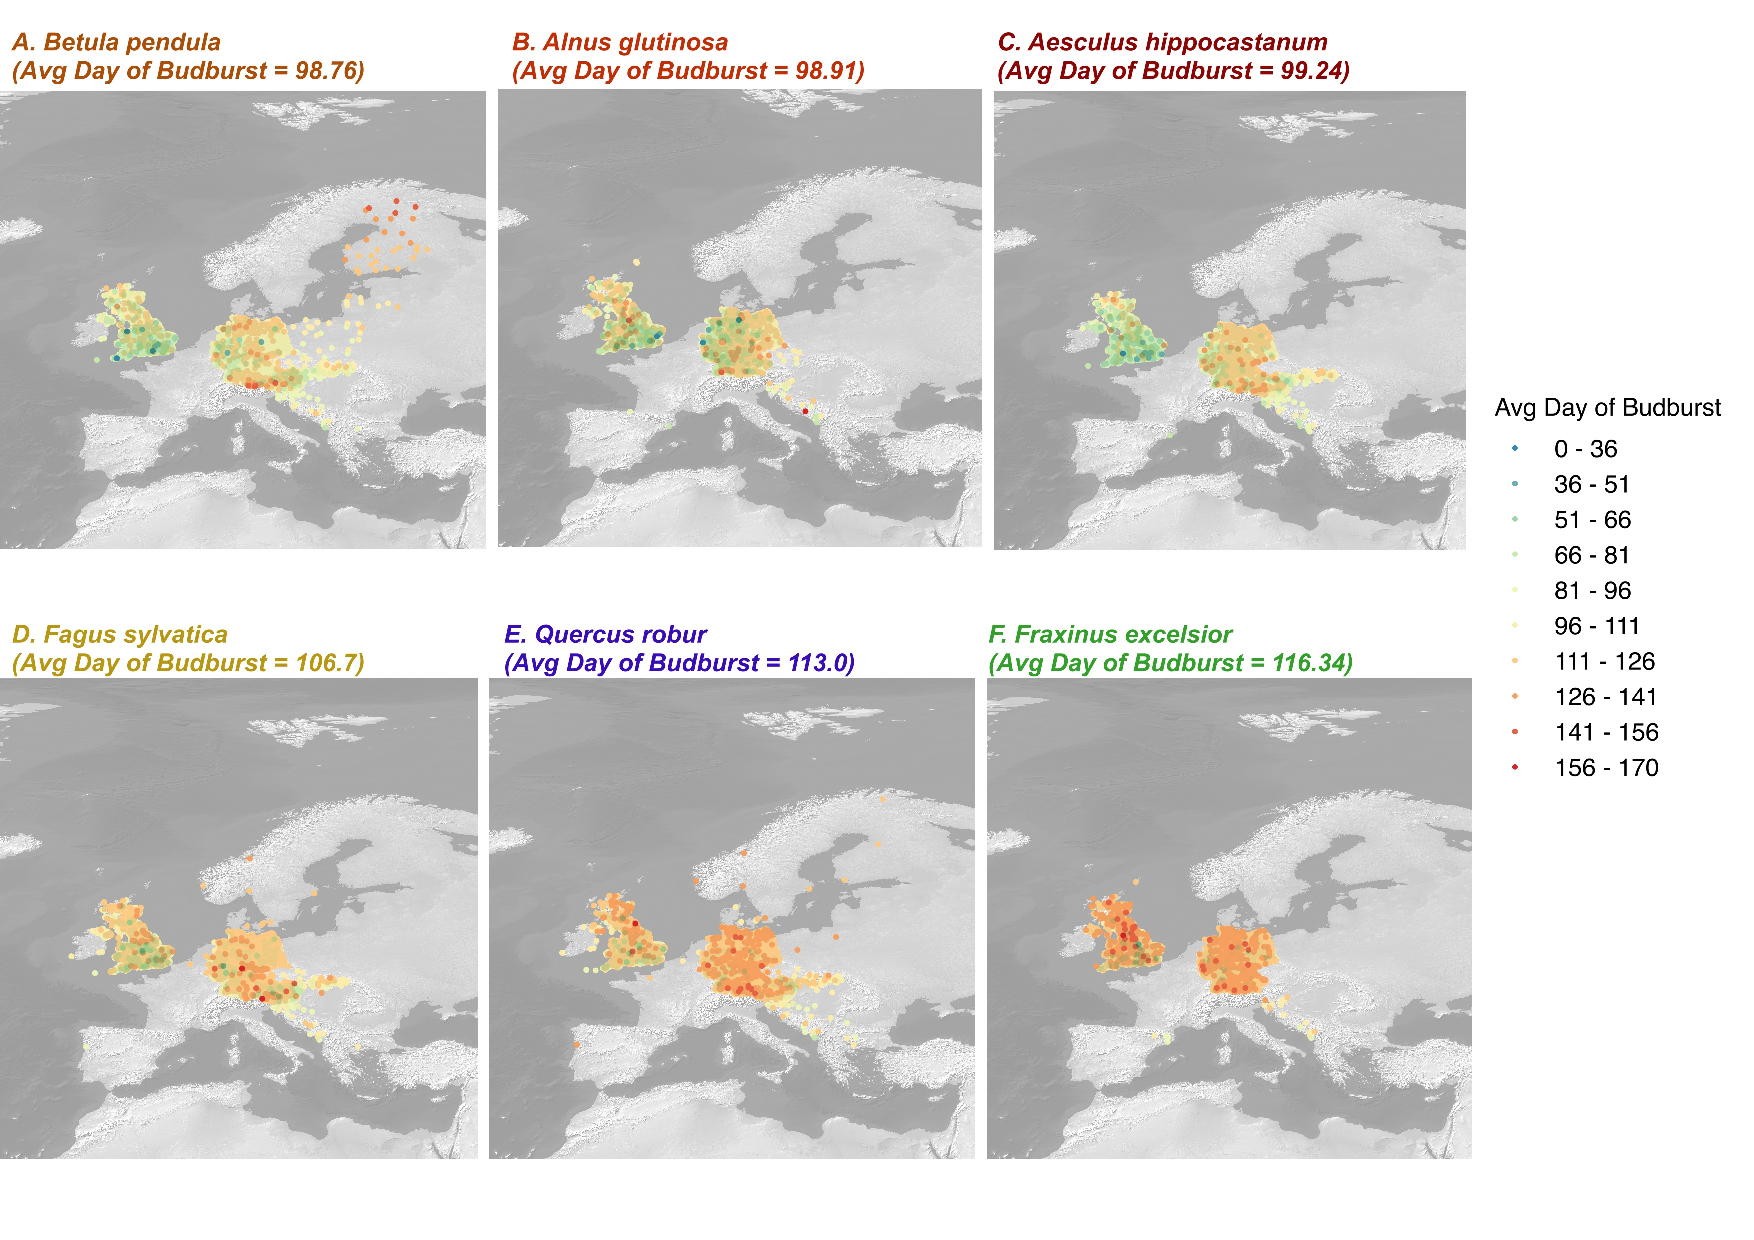
\includegraphics[width=14cm]{..//figures/BB_gis.pdf}
  -\caption{The average day of budburst is mapped by site for each species. Species are ordered by day of budburst starting with \textit{Betula pendula} as the earliest budburst date to \textit{Fraxinus excelsior}. Earlier budburst dates are blue and later budburst dates are in red. }\label{fig:bbmap}
  -\end{center}
  -\end{figure}}
  
{\begin{figure} [H]
  -\begin{center}
  -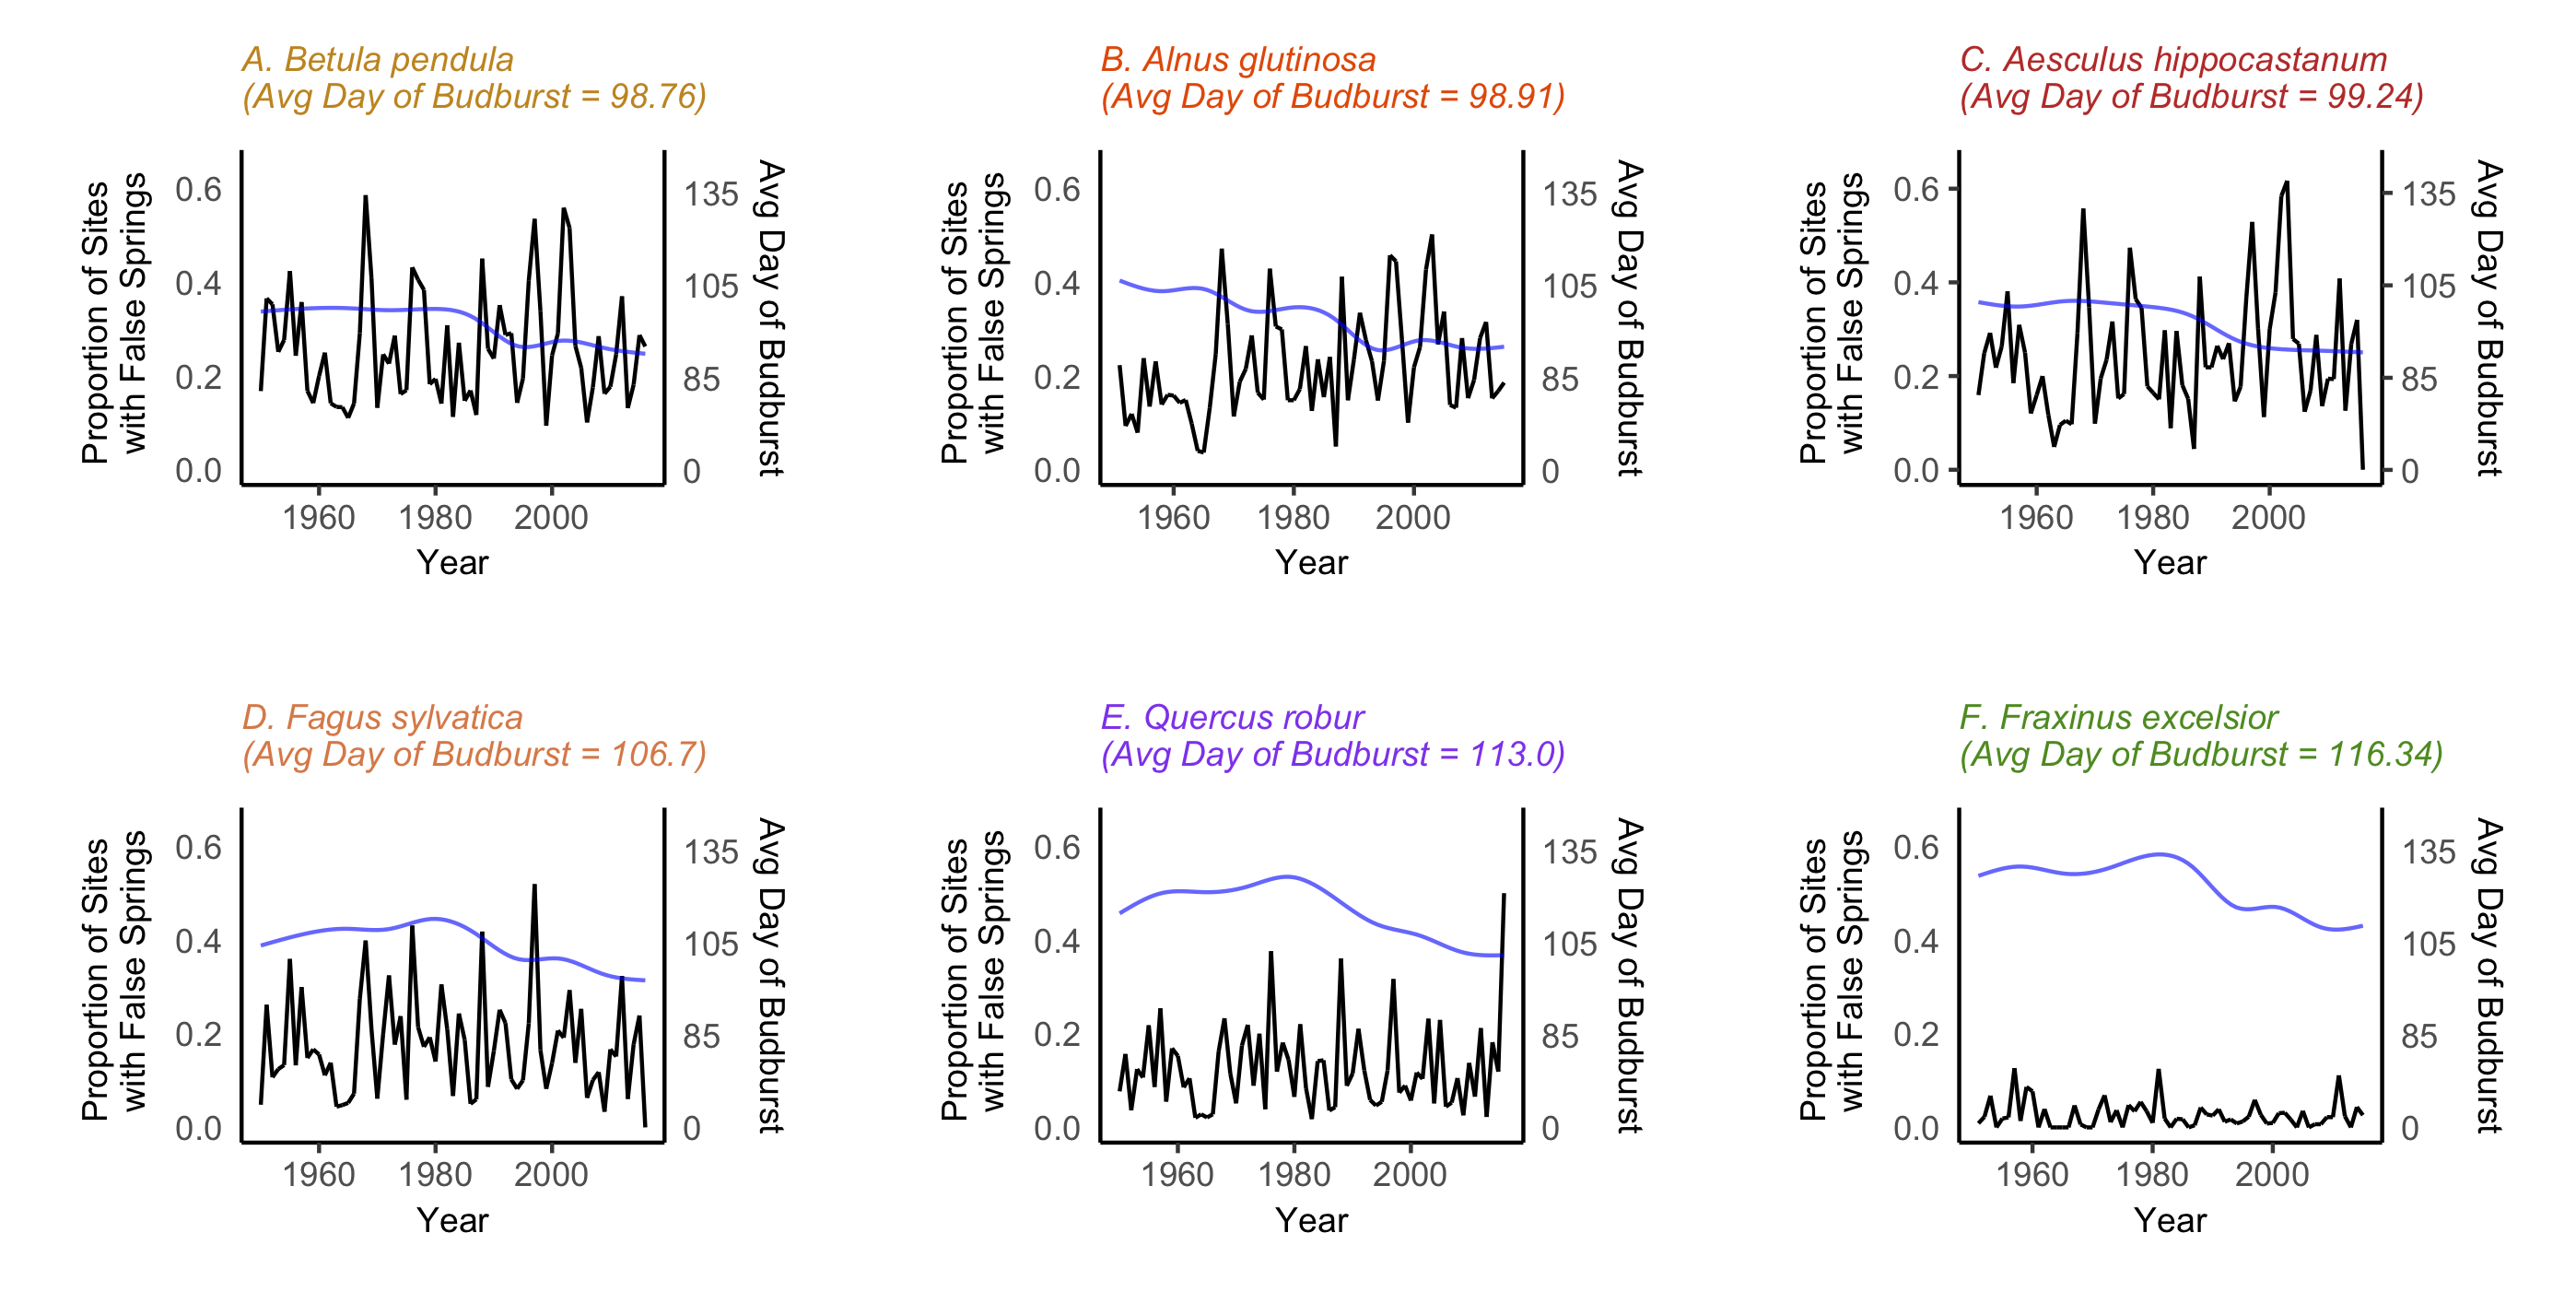
\includegraphics[width=16cm]{..//figures/PropSitesbyYrwBB.png}
  -\caption{The black line indicates the proportion of sites that had false spring conditions for each year across all species. The blue line is a smoothing spline, indicating the trend of average day of budburst for each year for each species. Species are ordered by average day of budburst, with the earliest being \textit{Betula pendula} and the latest being \textit{Fraxinus excelsior}.}\label{fig:fsprop}
  -\end{center}
  -\end{figure}}
  
{\begin{figure} [H]
  -\begin{center}
  -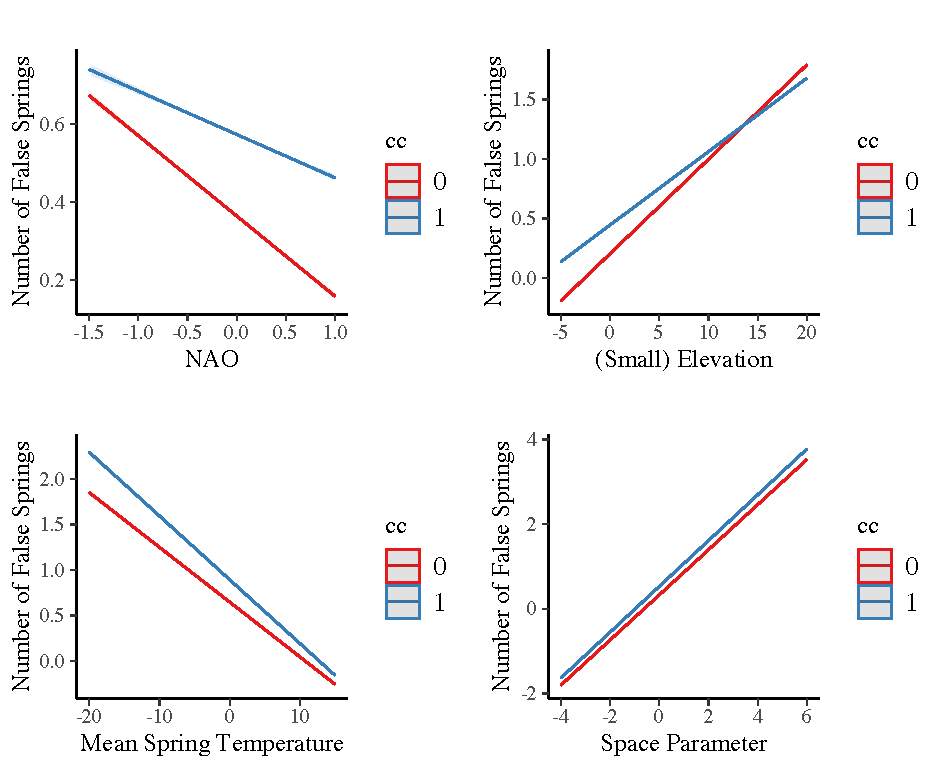
\includegraphics[width=12cm]{..//figures/InteractionPlots/InteractionPlots.pdf}
  -\caption{}\label{fig:hadbrms}
  -\end{center}
  -\end{figure}}
  
{\begin{figure} [H]
  -\begin{center}
  -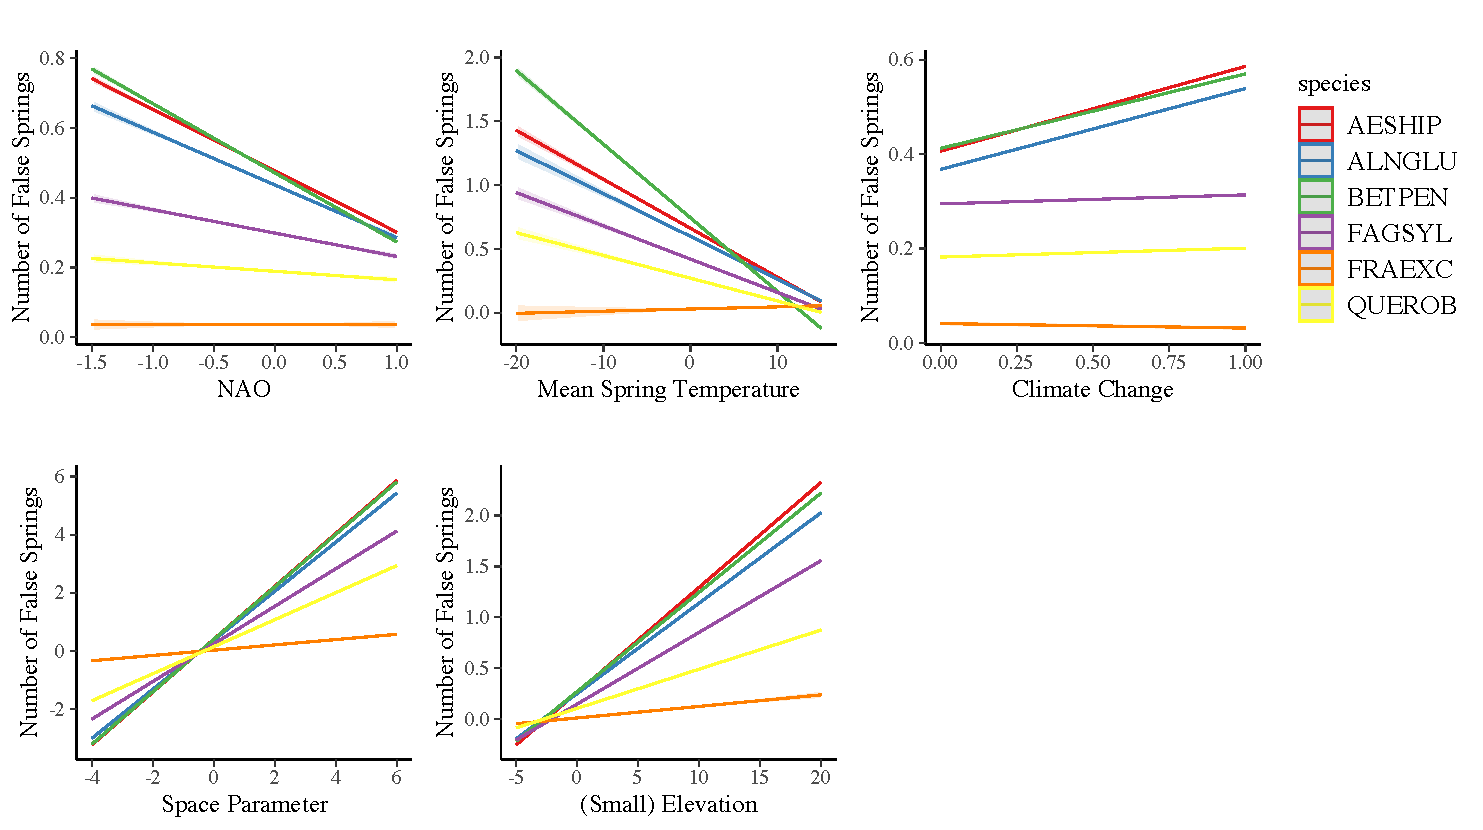
\includegraphics[width=16cm]{..//figures/InteractionPlots/SpeciesIntrxnPlots.pdf}
  -\caption{}\label{fig:maineffects}
  -\end{center}
  -\end{figure}}
  
\section*{Supplement: Tables and Figures}
{\begin{figure} [H]
  -\begin{center}
  -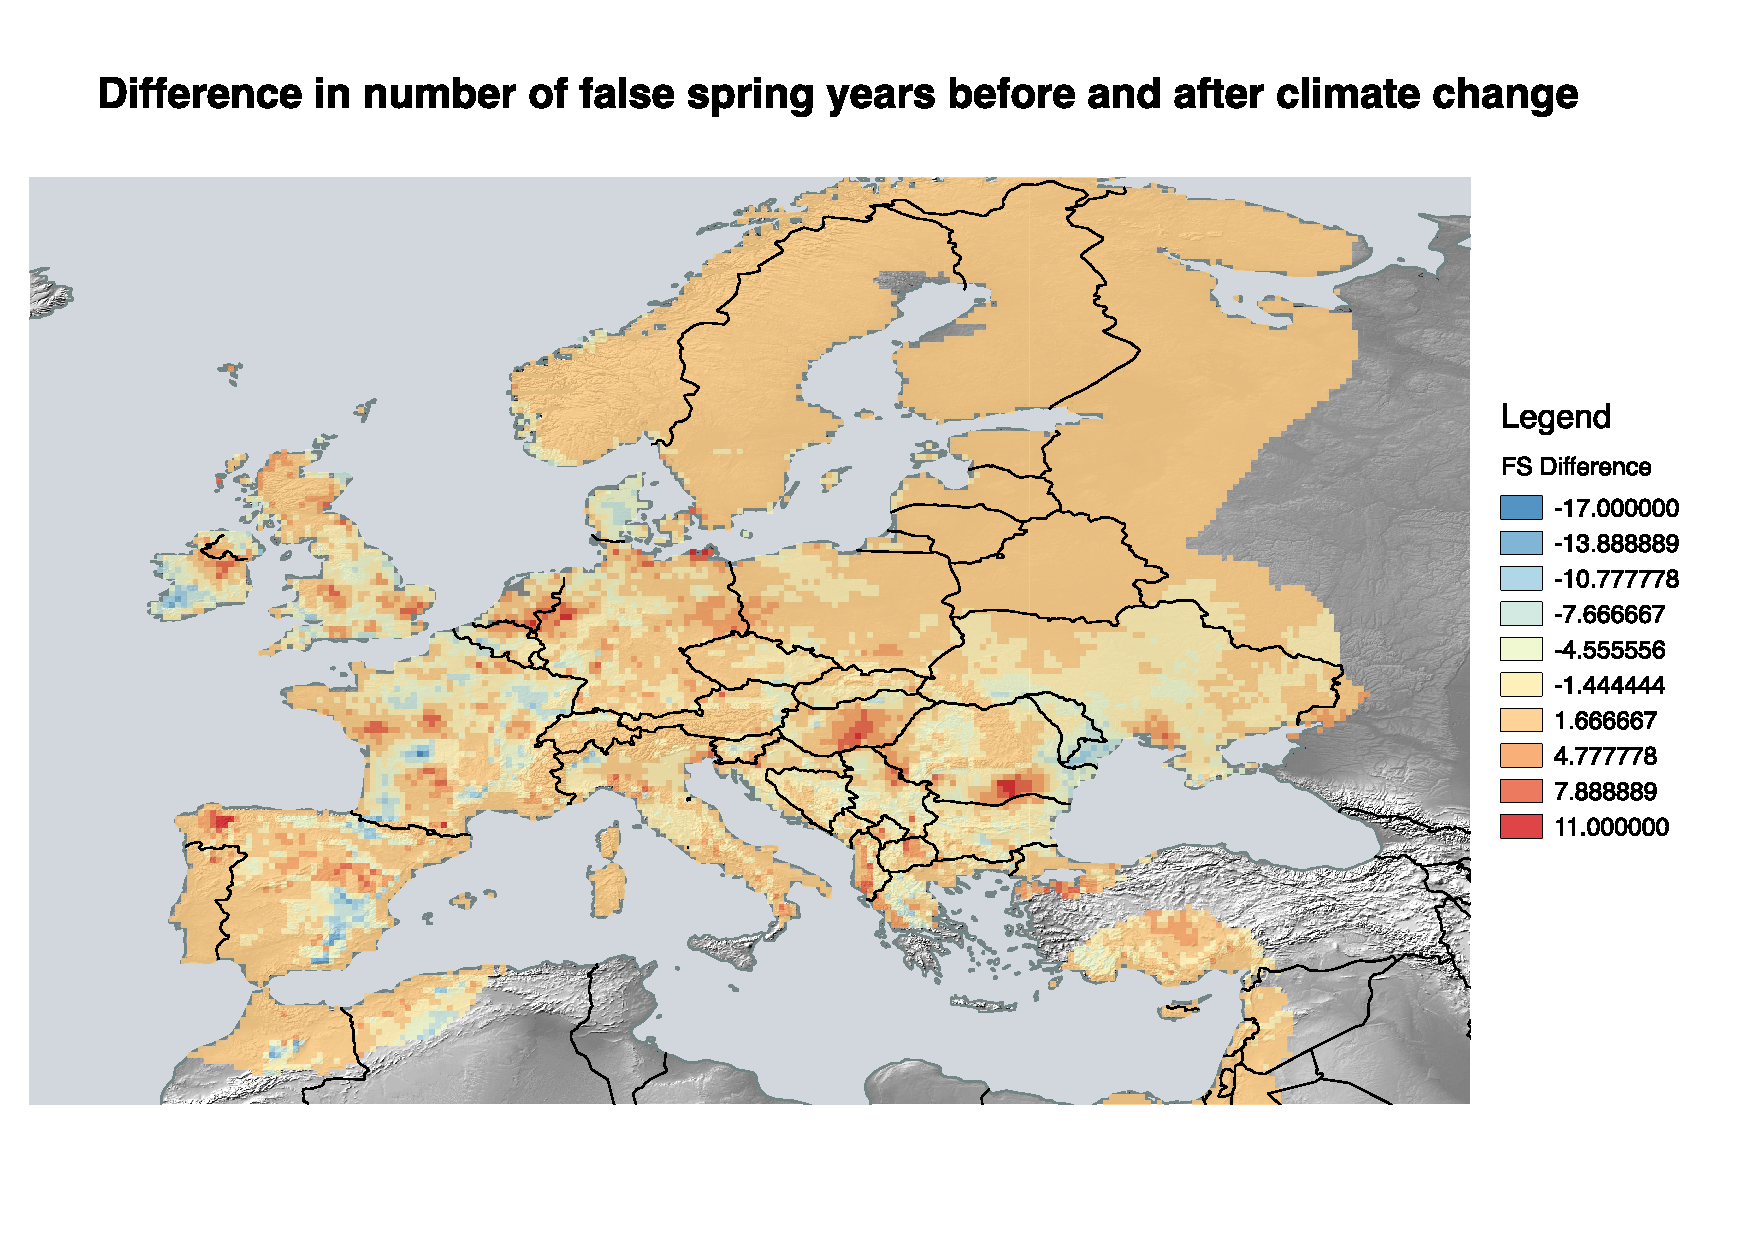
\includegraphics[width=12cm]{..//figures/FS_Diff.pdf}
  -\caption{Number of years with freezing events that occured before temperature shifts related to climate change began (1951-1983) as compared to after reported climate shifts (1984-2016). If temperatures fell below -2$^{\circ}$C between March 1 and June 30, a year with a spring freeze was tallied. Some regions experienced more years with spring freezes after climate change began, whereas other years experienced the same number or even fewer years with spring freezes. Regions that had more years with spring freezes after climate change began are blue and green and regions that had fewer freezes are depicted in red.}\label{fig:region}
  -\end{center}
  -\end{figure}}
  
\begin{center}
\captionof{table}{Data points collected for each species} \label{tab:spp} 
\begin{tabular}{c c c c}
\hline
\textbf{Species} & \textbf{Num. of Observations} & \textbf{Num. of Sites} & \textbf{Num. of Years} \\
\hline
\textit{Aesculus hippocastanum} & 216396 & 10158 & 66  \\
\hline
\textit{Alnus glutinosa} & 136991 & 6775 & 66 \\
\hline
\textit{Betula pendula} & 215729 & 10139 & 66 \\
\hline
\textit{Fagus sylvatica} & 185949 & 9099 & 66 \\
\hline
\textit{Fraxinus excelsior} & 143269 & 7327 & 65 \\
\hline
\textit{Quercus robur} & 184406  & 8811 & 66 \\
\end{tabular}
\end{center}
  
{\begin{figure} [H]
  -\begin{center}
  -\includegraphics[width=12cm]{..//figures/space_extremes.pdf}
  -\caption{Space parameter values are mapped for each location to elucidate patterns in the parameter values.}\label{fig:space}
  -\end{center}
  -\end{figure}}
  

\end{document}
